% Bedienungsanleitung für Clients

%\epigraph{	Your Time is precius. \newline Track your investments!}{\textit{Group 4}} %Raus mit dem kleinen Scherz??
\section{Bedienungsanleitung des Clients}
% So schön mit Bildern und so, erst bei fertiger Anwendung 

\begin{center}
	\textit{Your Time is precius. \newline Track your investments!}
\end{center}


TimeTracker bietet folgende Funktionen:
\begin{itemize}
	\item Time Tracking
	\item Anlegen und Löschen von Aktivitäten % durch User
	\item Tracking für verschiedene Aktivitäten
	\item Zuordnen mit Tags
	\item Abruf von Statistiken (Benutzer/Global)
\end{itemize}


Der Dienst ist online zu erreichen unter \url{http://iamtrent.de}

Lokale Installationen sind zu erreichen unter localhost:9123

\subsection{Build}

Zum Bild bitte folgende Zeilen Ausführen:
\begin{lstlisting}[language=bash]
	mvn clean install
	docker-compose -f docker/docker-compose.yml up -d
\end{lstlisting}

\subsection{Registrieren und Login }
 
 \begin{figure}[H]
 	\hspace{-1.5cm}
 	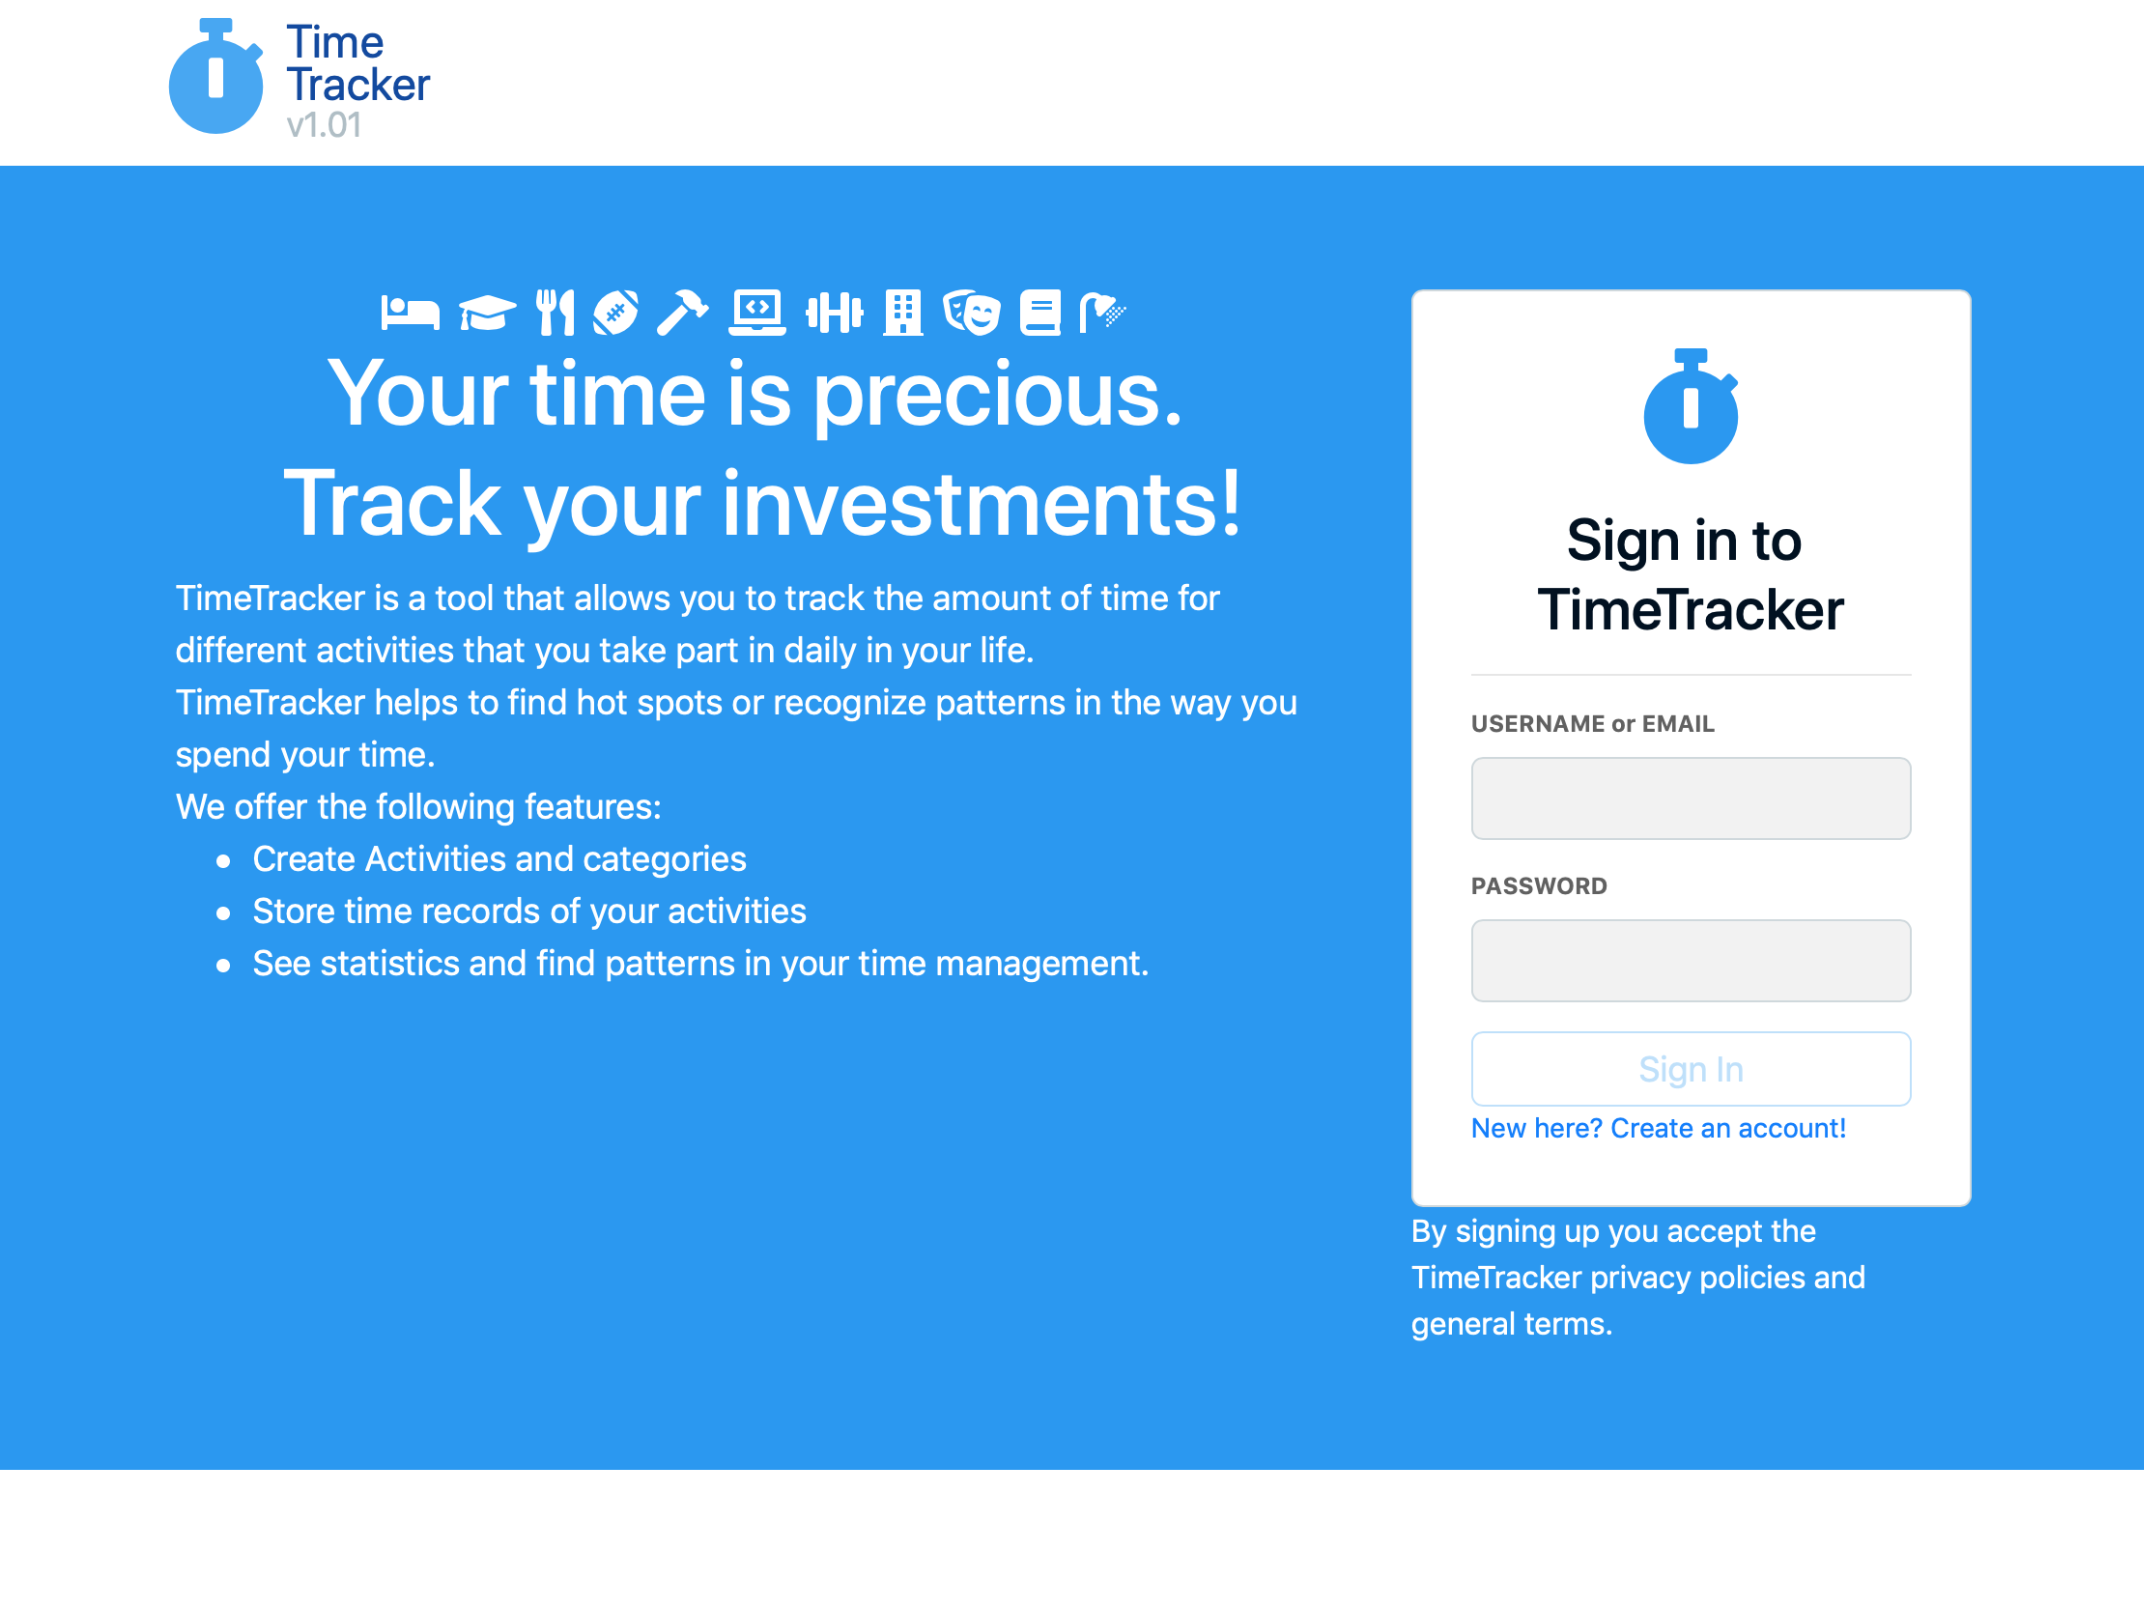
\includegraphics[width=1.15\linewidth]{login.png}
 	\caption{Login}
 	\label{fig:login}
 \end{figure}

Willkommen bei TimeTracker! Auf unserer Startseite (Abb. \ref{fig:login}) kannst du dich mit deinen Benutzerdaten einloggen.  
Du hast noch kein Benutzerkonto? Kein Problem, unterhalb des \textit{Sign In} Buttons ist ein Link, der zur Registrierung führt.
 

\begin{figure}[H]
	\hspace{-1.5cm}
	\centering
	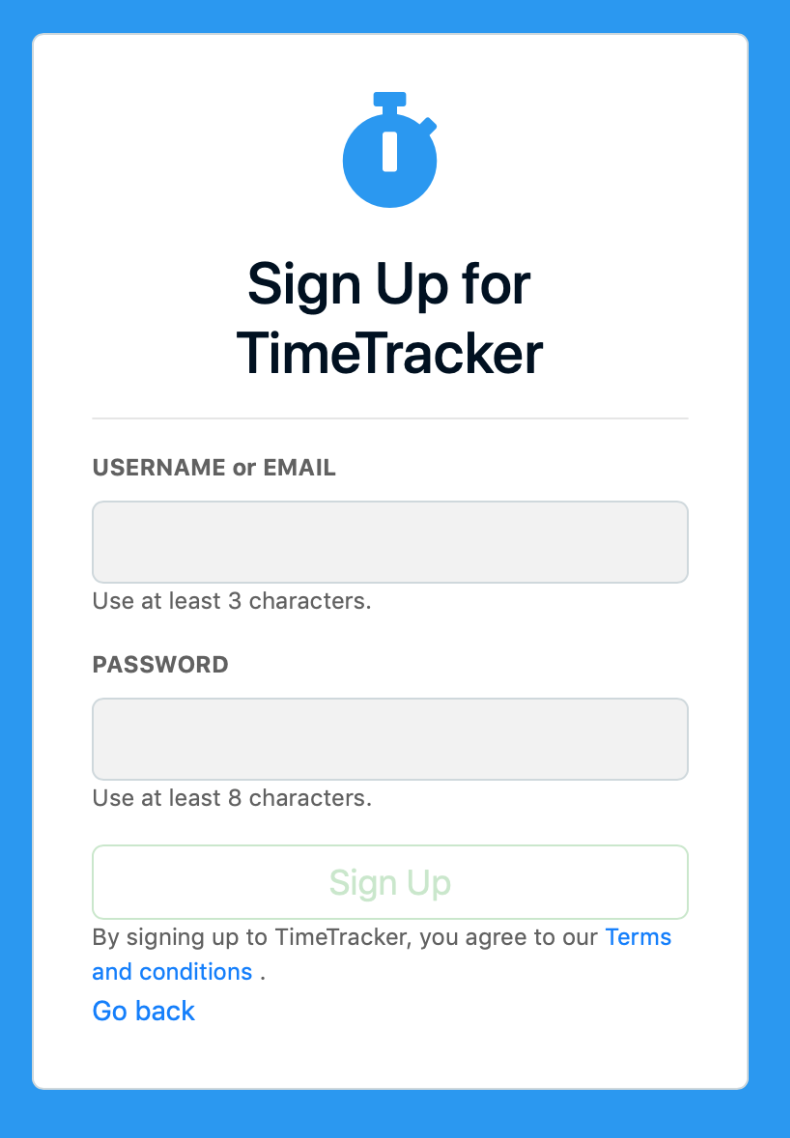
\includegraphics[scale=0.5]{register.png}
	\caption{Registrieren}
	\label{fig:register}
\end{figure}
%\newpage
%\begin{wrapfigure}{l}{0.5\textwidth}
%		\hspace{-1.5cm}
%		\centering
%		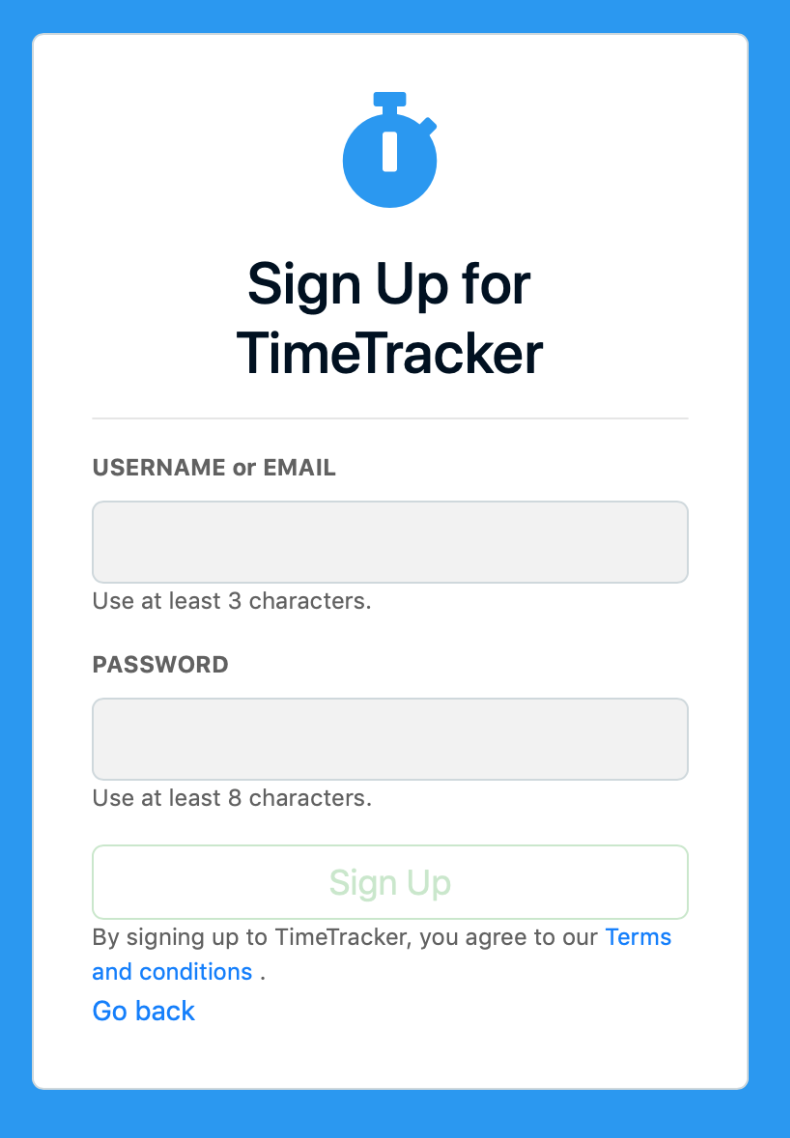
\includegraphics[width=0.38\textwidth]{register.png}
%		\caption{Registrieren}
%		\label{fig:register}
%\end{wrapfigure}

Um die zu registrieren musst du nur einen Usernamen oder eine Email, sowie ein Passwort eintragen. Beachte, dass das Passwort mindestens 8 Zeichen haben muss, vorher ist der Button nicht anklickbar! 
Nach dem du dich erfolgreich registriert hast wirst du wieder auf unsere Startseite (Abb. \ref{fig:login}) geleitet, wo du dich ab sofort mit deinen Nutzerdaten anmelden kannst. 

Wenn du einmal angemeldet bist kannst du dich jeder Zeit mit einem Klick auf \textit{Logout} oben rechts wieder abmelden.

\subsection{TimeTracken}

Wenn du dich das erste mal einloggst, sind noch keine Aktivitäten vorhanden. 
Aktivitäten sind die Aktionen, für die du deine Zeit trackst. 
Füge einfach eine neue Aktivität hinzu, in dem du auf \textit{+ New Aktivity} klickst (Abb. \ref{fig:no_activity}). 

\begin{figure}[H]
	\hspace{-1.5cm}
	\centering
	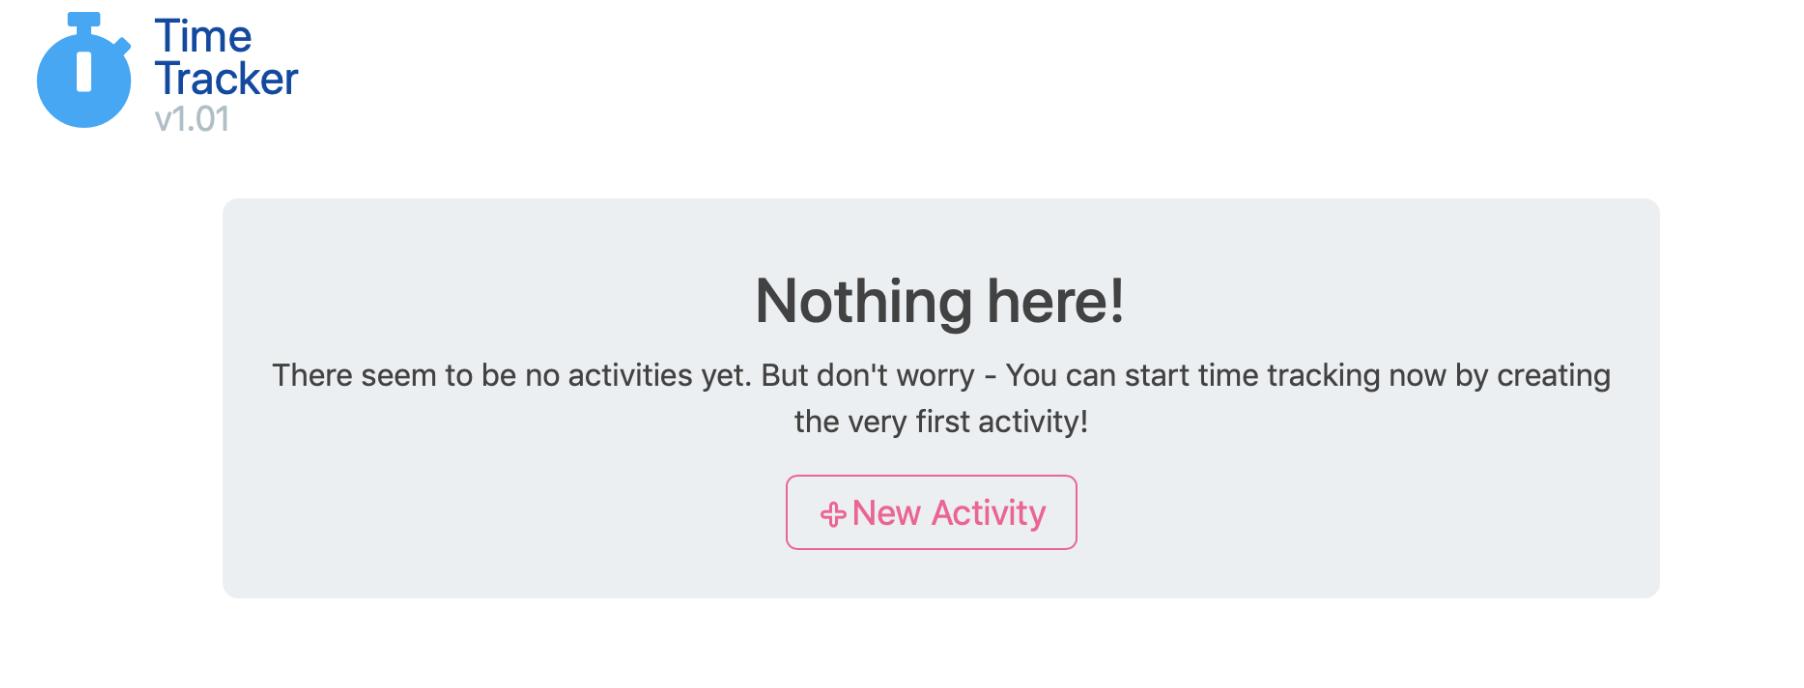
\includegraphics[scale=0.5]{no_activity.png}
	\caption{Keine Aktivitäten angelegt}
	\label{fig:no_activity}
\end{figure}

\begin{figure}[H]
	\hspace{-1.5cm}
	\centering
	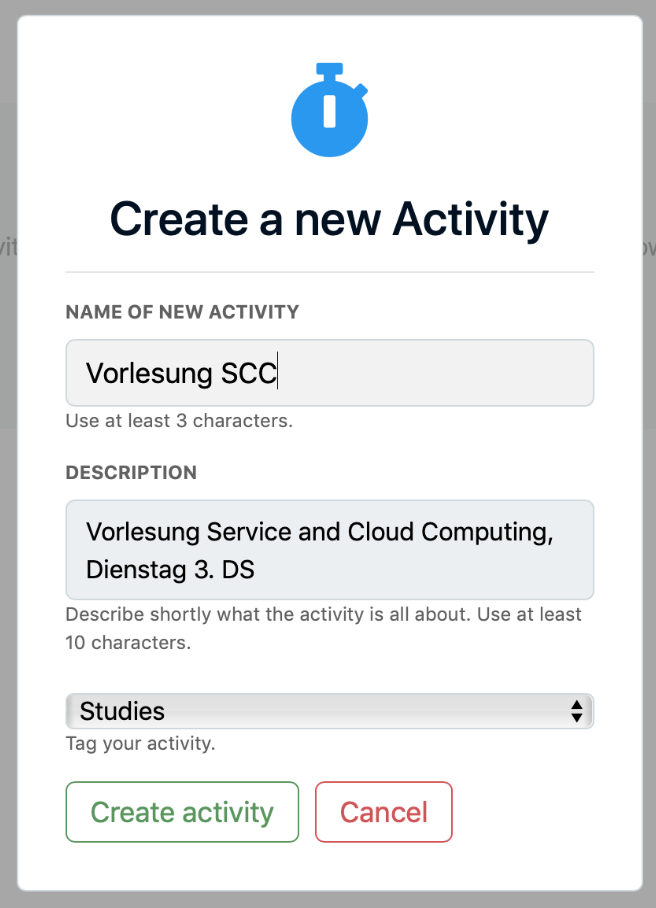
\includegraphics[scale=0.5]{create_activity.png}
	\caption{Aktivität anlegen}
	\label{fig:create_activity}
\end{figure}

Nun kannst du eine Aktivität anlegen (Abb. \ref{fig:create_activity}. 
Gibt ihr einen Namen und eine Beschreibung, damit du später weißt, wofür du sie angelegt hast. 
Der Name darf keine Umlaute wie \glqq Ä, Ö, Ü\grqq{}  enthalten und die Beschreibung muss mindeste 10 Zeichen lang sein. 
Danach verbindest du deine Aktivität mit einem Tag. Tags sind sowas wie Kategorien. 
Jede Aktivität hat ein Tag und dadurch eine Zuordnung zu einem deiner Lebensbereiche. 

Tags sind beispielsweise Studies, Sport und Relax. 
Mit Hilfe der Tags kannst du später schauen, wie viel Sport du gemacht hast, auch wenn du deine Zeit in den Aktivitäten "Schwimmen" und "Rad fahren" aufgenommen hast. 


\begin{figure}[H]
	\hspace{-1.5cm}
	\centering
	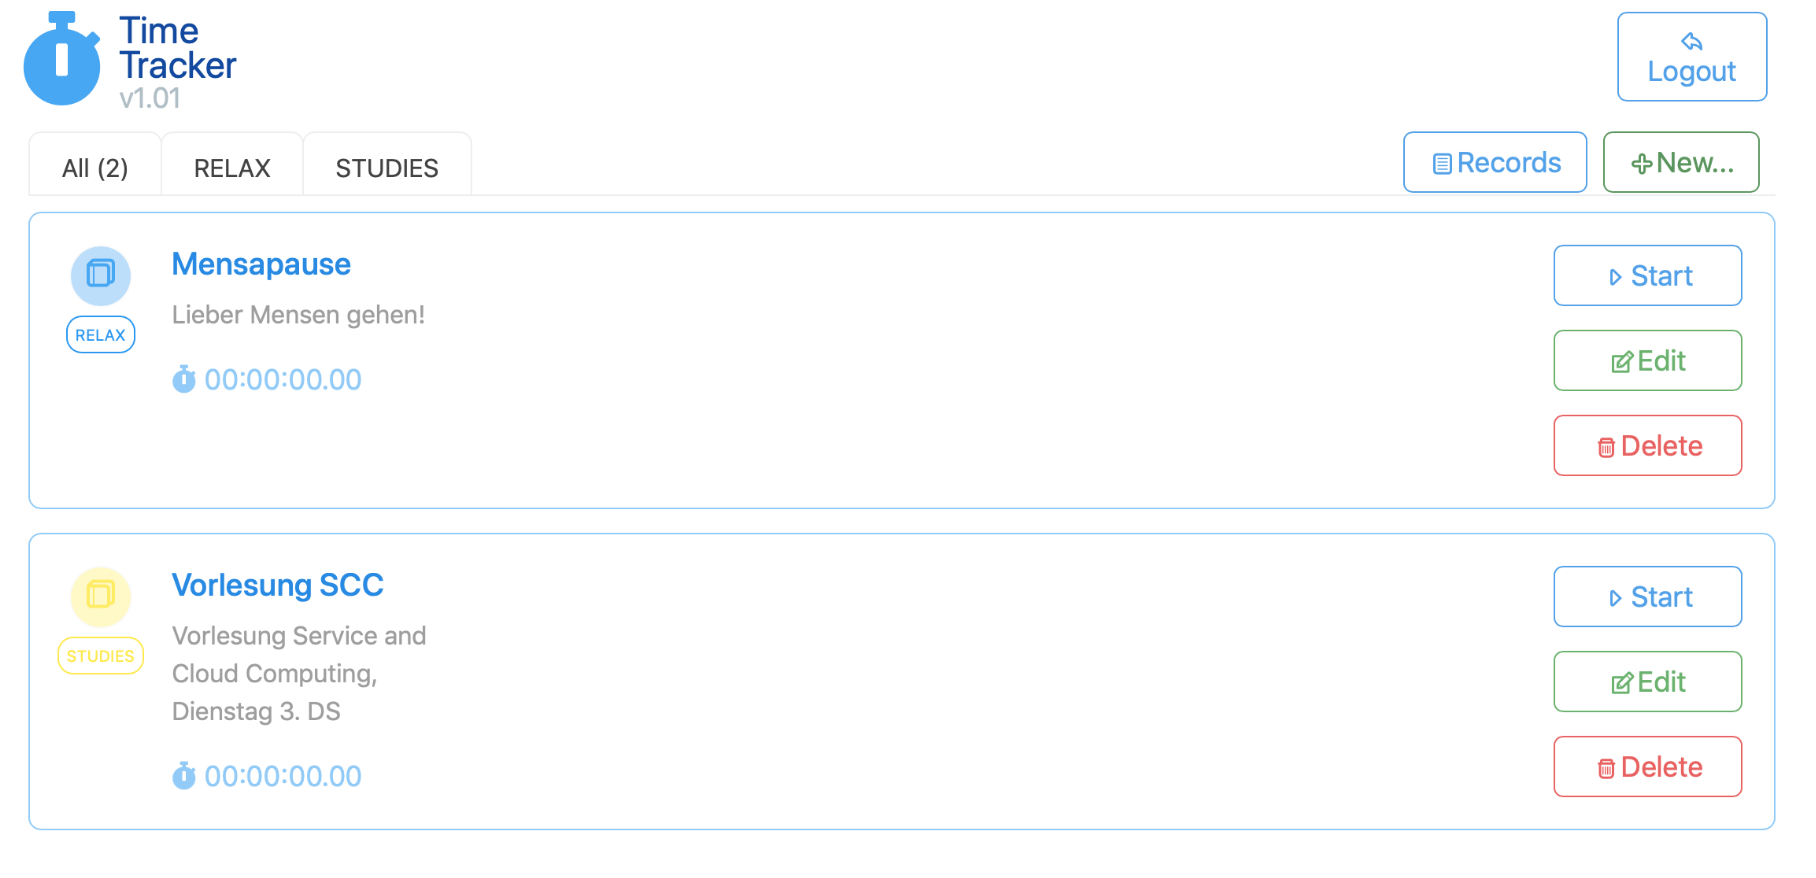
\includegraphics[scale=0.5]{activitys.png}
	\caption{Übersicht: Aktivitäten}
	\label{fig:activitys}
\end{figure}

Nun hast du Aktivitäten und eine Übersicht (Abb. \ref{fig:activitys}. Hier kannst du mit einem Klick auf  \textit{Start}  ein Record beginnen. Records sind die einzelnen Aufnahmen, die du machst. Zusammen addiert ergeben sie die gesamte Zeit, die du für eine Aktivität aufbringst. Wie du siehst, blinkt nun die Uhr und die Zeit läuft. 
Mit einem Klick auf den selben Button stoppst du das Tracking deiner Aktivität und beendest den Record. Du kannst dich zwischendurch auch abmelden oder von einem anderen Gerät aus einloggen, die Aufnahme geht einfach weiter. 

Mit dem Button \textit{+ New} kannst du weitere Aktivitäten anlegen und mit dem Button \textit{Delete} die jeweilige auch wieder löschen. In dem du auf \textit{Edit} klickst oder einfach auf den Titel/ die Beschreibung kannst du die Inhalte updaten. 

Über die Reiter oben kannst du deine Aktivität nach den von dir genutzten Tags filtern. 

\begin{figure}[H]
	\hspace{-1.5cm}
	\centering
	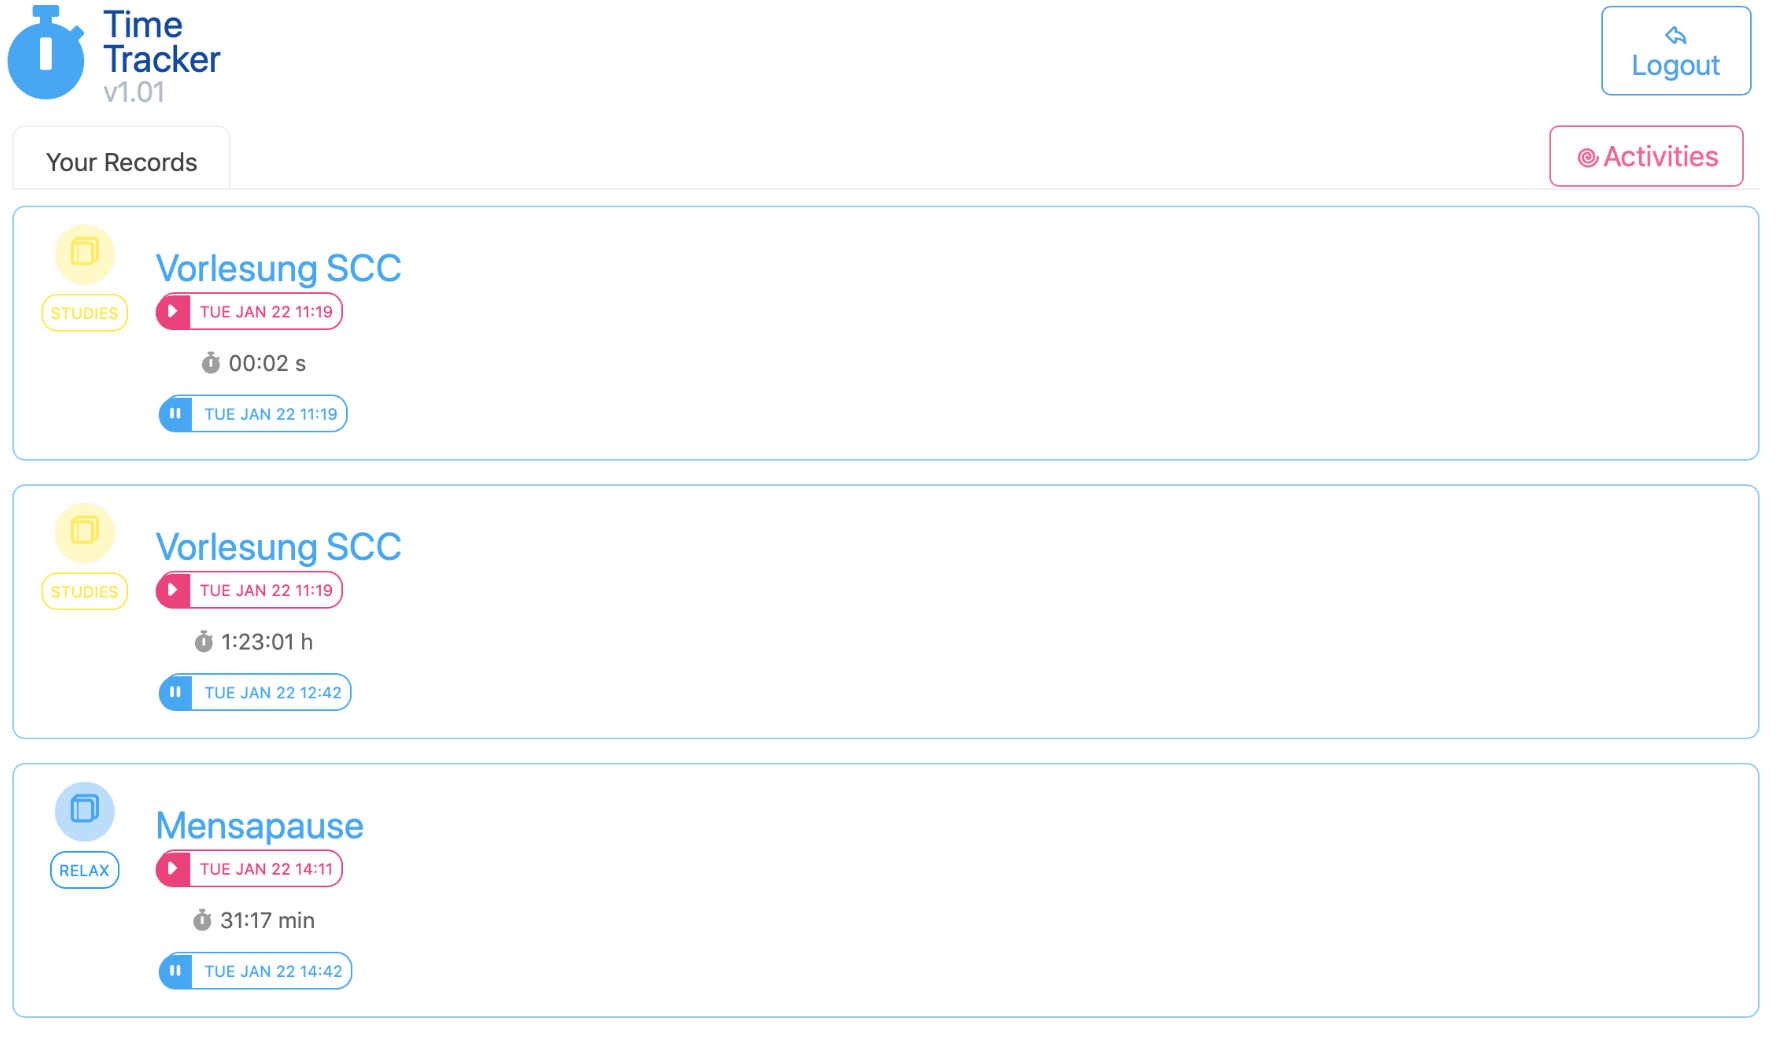
\includegraphics[scale=0.5]{records.png}
	\caption{Aufgenommene Records}
	\label{fig:records}
\end{figure}

Wenn du \textit{Records} anwählst kommst du zu einer Übersicht all deiner Zeitaufnahmen (Abb. \ref{fig:records}). Hier steht für welche Aktivität, von wann bis wann und wie lange die Aufnahmen war. 

